\chapter{Implementasi dan Pengujian}
\label{chap:implementasi}

Pada bab ini, akan dijelaskan hasil implementasi algoritma pada perangkat lunak ini. Cara dan
hasil pengujian perangkat lunak juga akan dijabarkan pada bab ini. Hasil pengujian tersebut akan
digunakan pengukuran tingkat keoptimalan dari proses optimisasi yang dilakukan algoritma ant
colony pada perangkat lunak.

\section{Implementasi Algoritma}

Perangkat lunak ini akan mampu membentuk objek dari kelas AntColonyAlgorithm yang bertugas
untuk mencari urutan pengerjaan / solusi yang optimal dari suatu kasus flow shop. Perangkat
lunak ini akan mampu menerima data masukan sebuah kasus flow shop dari sebuah file teks
dan membentuk objek AntColonyAlgorithm yang disesuaikan dengan data-data dari kasus yang
diberikan. Tampilan awal dari perangkat lunak akan tampak seperti pada gambar ~\ref{fig:tampilanawal}

\begin{figure}[H]
	\centering
	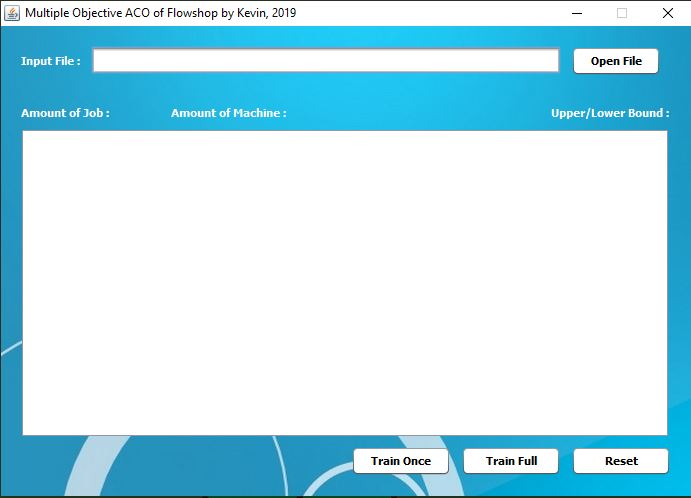
\includegraphics[scale=0.75]{TampilanAwal}
	\caption[Tampilan awal dari \textit{interface} perangkat lunak]{Tampilan awal dari \textit{interface} perangkat lunak}
	\label{fig:tampilanawal}
\end{figure}

Pada tampilan awal ini, pengguna belum dapat menjalankan proses optimisasi. Untuk dapat
menjalankan proses optimisasi, pengguna perlu memasukkan kasus flow shop terlebih dahulu
melalui tombol { \it "Open File"}. Tombol { \it "Open File"} tersebut akan membuka \textit{interface} baru seperti pada
gambar ~\ref{fig:pemilihankasus} Interface tersebut berguna untuk memilih file teks yang berisi kasus flow shop.

\begin{figure}[H]
	\centering
	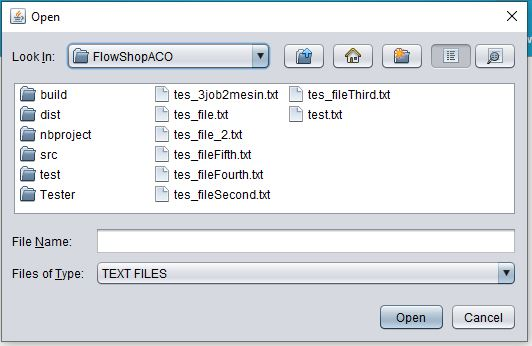
\includegraphics[scale=0.85]{PemilihanKasus}
	\caption[Tampilan \textit{interface} pemilihan kasus flow shop]{Tampilan \textit{interface} pemilihan kasus flow shop}
	\label{fig:pemilihankasus}
\end{figure}

Setelah kasus flow shop dipilih, perangkat lunak akan mengkonversi kasus tersebut menjadi
objek dari kelas Problem dan membentuk objek AntColonyAlgorithm berdasarkan data-data
kasus tersebut. Objek AntColonyAlgorithm tersebut akan membentuk objek dari kelas Pheromone-
Database dan AntColonySub yang akan membantu proses pencarian solusi optimal. Pembentukan
objek dari kedua kelas tersebut akan diatur oleh objek AntColonyAlgorithm agar sesuai dengan
kasus flow shop yang ingin dicari hasil optimalnya.

Objek dari kelas AntColonySub merepresentasikan sebuah kelompok semut yang akan disebar
pada saat proses pelatihan algoritma ant colony. Objek-objek AntColonySub tersebut akan mampu
melakukan pencarian solusi lokal secara bersama-sama. Banyaknya objek AntColonySub yang
dibentuk akan disesuaikan dengan banyaknya pekerjaan pada kasus flow shop yang dimasukkan.
Semakin banyak pekerjaan pada kasus flow shop yang diberikan, semakin banyak
pula objek AntColonySub yang dibentuk.

Setelah pengguna memasukkan kasus flow shop dan proses konversi kasus tersebut selesai,
pengguna dapat mulai melakukan proses optimisasi. Informasi-informasi penting mengenai kasus flow shop yang ingin dicari hasil optimalnya akan ditampilkan pada interface perangkat lunak
ini. Informasi mengenai banyaknya pekerjaan dan banyaknya mesin pada kasus flow shop akan ditampilkan pada \textit{interface} program. Nilai \textit{upper} dan \textit{lower bound} juga akan ditampilkan di \textit{interface} program. Tampilan interface tersebut akan tampak seperti gambar ~\ref{fig:setelahpemilihankasus} .

\begin{figure}[H]
	\centering
	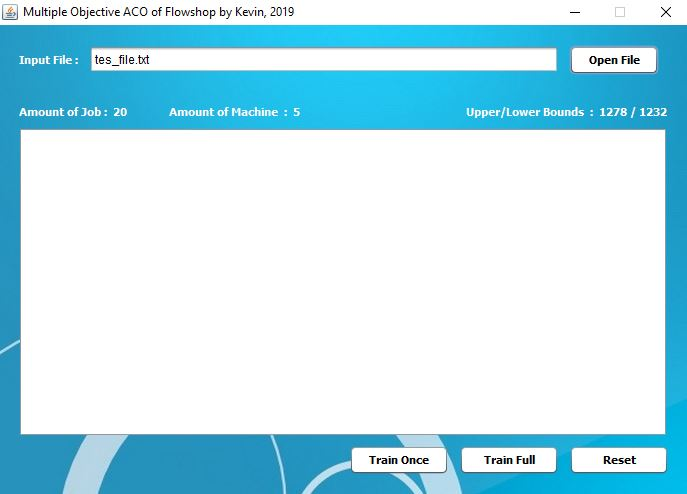
\includegraphics[scale=0.75]{SetelahPemilihanKasus}
	\caption[Tampilan \textit{interface} setelah pemilihan kasus flow shop]{Tampilan \textit{interface} setelah pemilihan kasus flow shop}
	\label{fig:setelahpemilihankasus}
\end{figure}

Pengguna dapat menggunakan beberapa cara dalam melakukan proses optimisasi. Untuk melakukan
proses optimisasi dengan menggunakan 1 kali fase pelatihan, pengguna dapat menekan
tombol \textit{"Train Once"}. Hasil dari proses optimisasi pada fase pelatihan ini akan ditampilkan pada
text area. Nilai-nilai pada fase pelatihan ini akan dicatat oleh objek AntColonyAlgorithm dalam
bentuk feromon dan akan mempengaruhi proses-proses optimisasi selanjutnya. Dengan dicatatnya
fase-fase pelatihan yang dilakukan, hasil proses optimisasi akan cenderung lebih baik dan semakin
mendekati solusi yang paling optimal.

Pengguna juga dapat melakukan proses optimisasi dengan melakukan fase pelatihan secara terus
menerus hingga suatu kondisi berhenti tercapai. Proses optimisasi tersebut dapat dilakukan dengan
menekan tombol \textit{"Train Full"}. Setiap fase pelatihan yang terjadi pada proses ini akan mempengaruhi
dengan fase pelatihan selanjutnya. Sama seperti fungsi pada tombol \textit{"Train Once"}, hasil dari proses
optimisasi pada setiap fase pelatihan yang terjadi akan ditampilkan pada text area.

\begin{figure}[H]
	\centering
	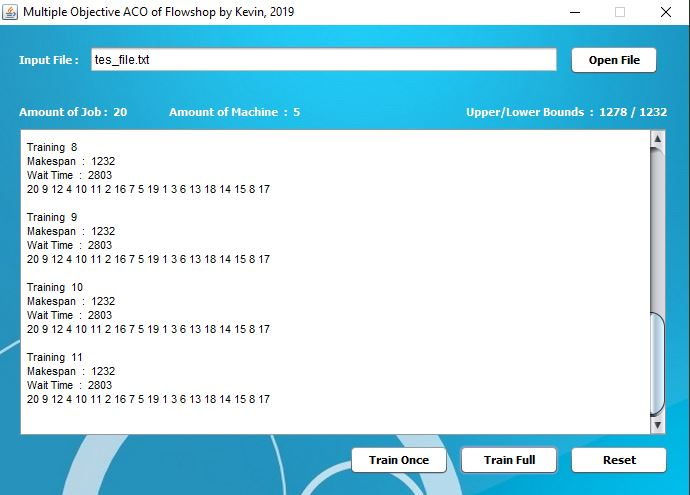
\includegraphics[scale=0.75]{SetelahOptimasi}
	\caption[Tampilan interface setelah beberapa proses optimisasi]{Tampilan interface setelah beberapa proses optimisasi}
	\label{fig:setelahoptimasi}
\end{figure}

Tampilan \textit{interface} setelah melakukan beberapa kali proses pelatihan / optimisasi akan terlihat
seperti gambar ~\ref{fig:setelahoptimasi} . Pengguna juga mampu mengulang proses optimisasi dari fase pelatihan pertama
dengan menekan tombol "Reset". Pengguna juga dapat memasukkan kasus flow shop baru
yang ingin dicari hasil optimalnya dengan menekan kembali tombol "Open File". Jika kasus flow shop yang baru telah dipilih, perangkat lunak akan membentuk ulang objek AntColonyAlgorithm
agar sesuai dengan kasus baru yang dipilih dan memulai kembali proses optimisasi dari fase pelatihan
pertama.

\section{Pengujian Fungsional}

Perangkat lunak ini akan memiliki beberapa fungsi, di antaranya : 
\begin{itemize}
	\item Mengkonversi \textit{file} teks menjadi kasus flow shop.
	\item Membentuk jalur secara acak.
	\item Menghitung nilai makespan dari kasus flow shop.
	\item Menghitung nilai wait time dari kasus flow shop.
	\item Membentuk feromon.
	\item Melakukan pelatihan dari algoritma ant colony.
\end{itemize}

Proses konversi \textit{file} teks sudah dapat dianggap berhasil setelah perangkat lunak mampu menampilkan
informasi banyaknya pekerjaan dan banyaknya mesin pada kasus flow shop.
Pengujian proses perhitungan nilai makespan dan nilai wait time akan dilakukan dengan menggunakan kasus flow 
shop yang sederhana. Kasus flow shop yang digunakan melibatkan 3 buah pekerjaan
dan 2 buah mesin. Kasus tersebut dijelaskan pada tabel ~\ref{tab:kasussederhana} :
% Table generated by Excel2LaTeX from sheet 'Sheet1'
\begin{table}[H]
	\centering
	\caption{Kasus Sederhana}
	\begin{tabular}{lrrr}
		& \multicolumn{1}{l}{J1} & \multicolumn{1}{l}{J2} & \multicolumn{1}{l}{J3} \\
		Mesin 1 & 5     & 4     & 6 \\
		Mesin 2 & 2     & 1     & 7 \\
	\end{tabular}%
	\label{tab:kasussederhana}%
\end{table}%

Dari kasus tersebut kemudian dimasukan ke dalam \textit{file} teks.
Maka hasil optimasi dari kasus tersebut ada pada gambar ~\ref{fig:hasilkasussederhana}

\begin{figure}[H]
	\centering
	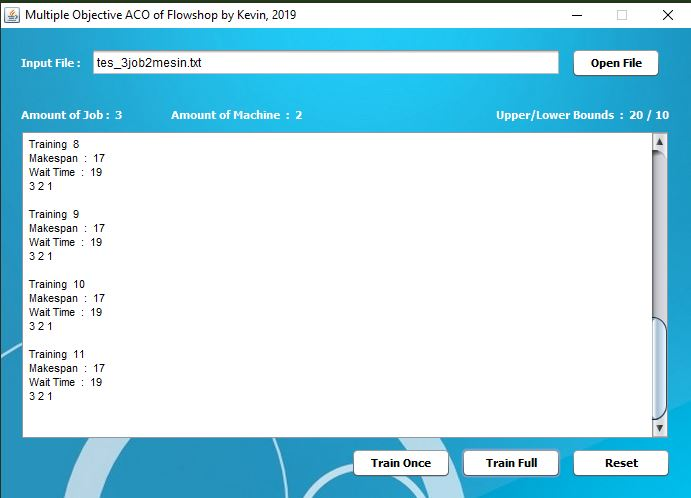
\includegraphics[scale=0.75]{HasilKasusSederhana}
	\caption[Hasil Kasus Sederhanai]{Hasil Kasus Sederhana}
	\label{fig:hasilkasussederhana}
\end{figure}

Perangkat lunak yang dibuat sudah mampu menghasilkan nilai makespan 17 dan nilai wait time 19 dari kasus tersebut. Jalur secara acak juga sudah berhasil ditampilkan oleh perangkat lunak. Untuk membuktikan jika nilai makespan yang dihasilkan sudah benar maka akan dibuktikan lewat perhitungan pada gambar ~\ref{fig:hasilhitungmanual}

\begin{figure}[H]
	\centering
	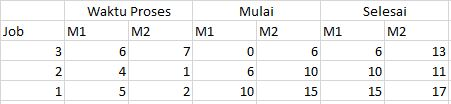
\includegraphics[scale=0.85]{HitungManual}
	\caption[Hasil Hitung Manual]{Hasil Hitung Manual}
	\label{fig:hasilhitungmanual}
\end{figure}

Dari hasil tersebut nilai makespan yang dihasilkan adalah 17 sehingga sudah sesuai dengan hasil dari perangkat lunak. Sedangkan untuk nilai wait time
sulit untuk dilakukan pemantauan secara langsung, pembuktian yang paling mungkin dilakukan adalah menganalisa lebih lanjut kode program pada kelas Flow
Shop dimana terdapat \textit{method} perhitungan wait time. Setelah proses pelatihan selesai, penambahan nilai feromon akan dilakukan oleh perangkat lunak.
Nilai feromon yang dihasilkan oleh perangkat lunak ditunjukan pada  tabel ~\ref{tab:nilaiferomon}.
% Table generated by Excel2LaTeX from sheet 'Sheet1'
\begin{table}[H]
	\centering
	\caption{Nilai Feromon}
	\begin{tabular}{rrr}
		0     & 42    & 28 \\
		21    & 0     & 49 \\
		98    & 56    & 0 \\
	\end{tabular}%
	\label{tab:nilaiferomon}%
\end{table}%

Tabel ~\ref{tab:nilaiferomon} merupakan tabel nilai feromon yang dihasilkan dari kasus flow shop dengan 3 buah pekerjaan. Pada tabel tersebut dapat dilihat bahwa terdapat beberapa indeks dengan nilai yang jauh lebih besar dibandingkan dengan indeks-indeks yang lain. Indeks-indeks feromon tersebut merupakan indeks-indeks feromon yang membantu pembentukan suatu solusi dan solusi tersebut merupakan solusi yang dianggap paling optimal pada saat ini.


\section{Eksperimen}

Pada bagian ini akan dijelaskan mengenai tata cara yang digunakan untuk melakukan eksperimen
dan informasi apa saja yang diambil dari eksperimen tersebut. Hasil data dan analisa dari eksperimen
tersebut juga akan dijelaskan.

\subsection{Spesifikasi Perangkat Keras}

Perangkat lunak ini dibangun menggunakan beberapa spesifikasi perangkat keras sebagai berikut :
\begin{enumerate}
	\item  Processor : Intel(R) Core(TM) i5-5200U 2.20GHz 
	\item  Operating System : Windows 10 Pro 64-bit (10.0, Build 18362) 
	\item  Memory: 4096MB RAM
\end{enumerate}

\subsection{Lingkungan Implementasi Perangkat Lunak}

Perangkat lunak ini dibangun menggunakan beberapa spesifikasi perangkat lunak sebagai berikut :
\begin{enumerate}
	\item NetBeans IDE versi 8.2
	\item Bahasa pemrograman Java (jdk) versi 1.7
	
\end{enumerate}

\subsection{Cara Eksperimen}

Eksperimen ini akan mencari tahu pengaruh jumlah semut, banyaknya pekerjaan, dan banyaknya mesin terhadap hasil optimisasi yang diberikan oleh algoritma ant colony. Eksperimen ini juga akan mencari tahu apakah algoritma ant colony ini sudah berjalan dengan benar. Data masukan yang akan digunakan berasal dari \textit{benchmark tailard}. Data kasus yang digunakan dibatasi pada 20 pekerjaan dan 50 pekerjaan saja. Proses eksperimen akan dilakukan dengan memasukkan \textit{file} teks dari beberapa jenis kasus flow shop yang disediakan oleh \textit{tailard}. Masing-masing jenis kasus akan dibedakan berdasarkan banyaknya pekerjaan dan banyaknya mesin. Eksperimen akan melakukan optimisasi pada 10 kasus yang berbeda untuk setiap jenis kasus yang ada .

Proses eksperimen akan melakukan proses optimisasi untuk setiap data kasus sebanyak 5 kali.
Hal ini dilakukan untuk mendapatkan rata-rata nilai makespan dan rata-rata nilai wait time yang didapatkan dari optimisasi
sebuah data kasus. Pada eksperimen akan dilakukan optimisasi dengan menggunakan tombol \textit{"Train Full"} secara berulang hingga fase pelatihan telah menghasilkan solusi yang sama sebanyak 10 kali. Pada setiap kasus, eksperimen akan melakukan optimisasi dengan 2 jumlah semut yang berbeda.
Proses optimisasi ini akan melakukan proses pelatihan algoritma ant colony dengan melibatkan n
dan n*2 semut, di mana n adalah banyaknya pekerjaan pada kasus flow shop yang dipilih.
Jumlah semut tersebut digunakan dengan asumsi bahwa jumlah semut yang disebar pada setiap fase pelatihan mempengaruhi
tingkat kompleksitas dari algoritma ant colony. Semakin rumit kasus, maka semakin lama waktu yang dibutuhkan untuk proses optimisasi.

Hasil eksperimen yang akan dicatat adalah nilai makespan yang dihasilkan, urutan pengerjaan /
solusi yang menghasilkan nilai makespan tersebut, nilai wait time yang dihasilkan, dan pada fase pelatihan ke berapa solusi tersebut
didapatkan. Hasil dari nilai makespan yang diberikan akan dibandingkan dengan nilai \textit{lower bound} dari \textit{tailard}. Nilai \textit{lower} itu sendiri akan dianggap sebagai nilai makespan target. Jika nilai makespan yang dihasilkan semakin mendekati nilai \textit{lower bound}, maka semakin baik pula penilaian terhadap tingkat optimisasi algoritma ini.

\subsection{Hasil Eksperimen}

\begin{figure}[H]
	\centering
	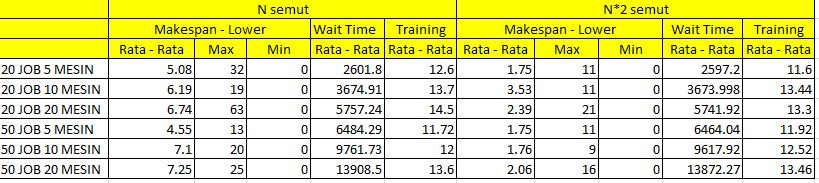
\includegraphics[scale=0.75]{HasilEksperimen3}
	\caption[Hasil Eksperimen]{Hasil Eksperimen}
	\label{fig:hasileksperimen}
\end{figure}

Gambar ~\ref{fig:hasileksperimen} di atas berisi tabel data hasil eksperimen yang telah dilakukan. Untuk setiap kasus telah dilakukan perhitungan rata-rata selisih nilai makespan dengan nilai \textit{lower bound} dari 5 kali pengulangan proses optimisasi. Nilai-nilai tersebut kemudian akan dikelompokkan berdasarkan banyaknya semut yang disebar dan jenis kasus flow shop yang menghasilkannya. Selain makespan dicatat juga nilai rata - rata wait time dari setiap kasus. Jenis dari suatu kasus dapat didefinisikan berdasarkan banyaknya pekerjaan dan mesin pada setiap tahap proses dari suatu kasus. Selain itu nilai rata - rata dari proses pelatihan untuk mendapatkan solusi juga dicatat pada eksperimen

\subsection{Analisa Hasil Eksperimen}

Berdasarkan hasil eksperimen, dapat dilihat bahwa algoritma ant colony mampu menghasilkan nilai
makespan yang paling optimal. Hal ini dapat dilihat dari data minimal dari nilai minimal pada
selisih makespan dengan \textit{lower bound}. Nilai selisih 0 menunjukkan bahwa algoritma ant colony
berhasil selalu mendapatkan nilai makespan yang paling optimal dari 5 kali proses optimisasi suatu
kasus yang sama. 

Nilai selisih makespan dengan \textit{lower bound} akan semakin besar jika kasus yang
ingin dioptimisasi semakin rumit. Pada optimisasi kasus flow shop dengan 50 buah pekerjaan,
nilai selisih yang dihasilkan cenderung sangat besar. Jika dibandingkan dengan nilai selisih pada
optimisasi kasus flow shop dengan 20 buah pekerjaan. Begitu juga dengan nilai wait time semakin rumit suatu kasus maka semakin tinggi pula nilai wait time yang dihasilkan. Semakin banyak
pekerjaan yang ada pada kasus flow shop, maka tingkat keoptimalan dari hasil optimisasi algoritma ant colony ini akan semakin lama untuk dicapai.

Cara untuk menambah tingkat keoptimalan hasil optimisasi dapat dilakukan dengan menambah
banyak semut yang disebar pada fase pelatihan. Hal ini dapat dilihat pada gambar  ~\ref{fig:hasileksperimen} , pada
hasil optimisasi kasus-kasus dengan jumlah semut yang berbeda. Hasil nilai selisih yang dihasilkan
dengan \textbf{n*2} semut pada setiap fase pelatihan selalu bernilai lebih kecil jika dibandingkan dengan
yang dihasilkan oleh \textbf{n} semut. Dari hal tersebut dapat dilihat bahwa semakin banyak semut yang
disebar, maka hasil optimisasi yang dihasilkan juga akan cenderung lebih mendekati nilai yang
paling optimal.

Banyaknya semut yang disebar juga mempengaruhi banyaknya fase pelatihan yang dibutuhkan
untuk mencapai hasil optimal. Banyaknya fase pelatihan yang dilalui relatif lebih sedikit jika proses
optimisasi dilakukan dengan jumlah semut yang lebih banyak. Di sisi lain, semakin rumit suatu
kasus yang ingin dioptimisasi, maka semakin banyak pula fase pelatihan yang perlu dilalui untuk
mencapai hasil yang optimal.

Cukup sulit untuk membuktikan bahwa algoritma ini telah bekerja sesuai dengan yang diinginkan.
Algoritma ant colony sulit untuk dianalisa secara teoritis, karena membentuk solusi secara
acak. Nilai-nilai feromon yang mempengaruhi pembentukan solusi tersebut juga selalu mengalami perubahan.
Cara untuk menganalisa algoritma ini hanya dengan menggunakan cara eksperimental dengan
mengambil beberapa sampel hasil solusi.

% Table generated by Excel2LaTeX from sheet 'Hasil'
\begin{table}[H]
	\centering
	\caption{Sampel hasil solusi}
	\begin{tabular}{cccc}
		\toprule
		Nilai Makespan & Wait Time & Training & Urutan Pengerjaan \\
		\midrule
		1185  & 2323  & 11    & 9 19 3 10 17 14 15 11 20 4 16 18 6 5 8 2 1 12 7 13  \\
		\midrule
		1183  & 2299  & 12    & 10 7 5 11 8 9 15 14 19 3 6 17 18 16 20 4 12 2 1 13  \\
		\midrule
		1181  & 2395  & 19    & 15 5 7 14 4 3 17 1 6 13 16 12 20 9 8 19 2 10 18 11  \\
		\midrule
		1185  & 2316  & 13    & 4 6 12 17 9 1 5 10 19 20 8 11 2 3 16 15 14 18 7 13  \\
		\midrule
		1180  & 2435  & 11    & 9 18 13 4 7 11 15 2 19 3 16 17 1 14 20 12 8 10 5 6  \\
		\bottomrule
	\end{tabular}%
	\label{tab:sampelsolusi}%
\end{table}%

Tabel ~\ref{tab:sampelsolusi} di atas merupakan hasil pengujian salah satu kasus flow shop dengan 20 buah pekerjaan dan 5 mesin. Hasil optimisasi di atas dapat dijadikan data sampel untuk membuktikan bahwa algoritma ant colony yang diaplikasikan sudah bekerja dengan benar. Hal ini dapat dilihat dari dipilihnya
pekerjaan 13 sebagai pekerjaan untuk dikerjakan terakhir pada tiga solusi yang didapatkan. Pekerjaan 9 juga cenderung untuk dikerjakan pertama kali.

Dalam satu kasus flow shop, algoritma ant colony akan cenderung mengarahkan dirinya untuk membentuk sebuah solusi yang sama. Solusi yang dijadikan tujuan tentu saja merupakan solusi yang paling optimal dari kasus flow shop tersebut. Pada perangkat lunak ini, algoritma ant colony akan berusaha membentuk urutan-urutan pekerjaan yang terbaik berdasarkan prioritas diambilnya suatu pekerjaan setelah diambilnya pekerjaan yang lain. Jika fase pelatihan dari hasil proses pengujian tersebut dilanjutkan, solusi yang dihasilkan kemungkinan besar akan semakin mirip bahkan dapat serupa.






